\chapter{Fission Bank}

\section{Algorithms}
\label{sec:algorithms}

\subsection{Traditional Algorithm}

Monte Carlo particle transport codes commonly implement a SPMD model
by having one master process that controls the scheduling of work and
the remaining processes wait to receive work from the master, process
the work, and then send their results to the master at the end of the
simulation (or a source iteration in the case of an eigenvalue
calculation). This idea is illustrated in Figure
\ref{fig:master-slave}.
\begin{figure}[h!]
  \centering
  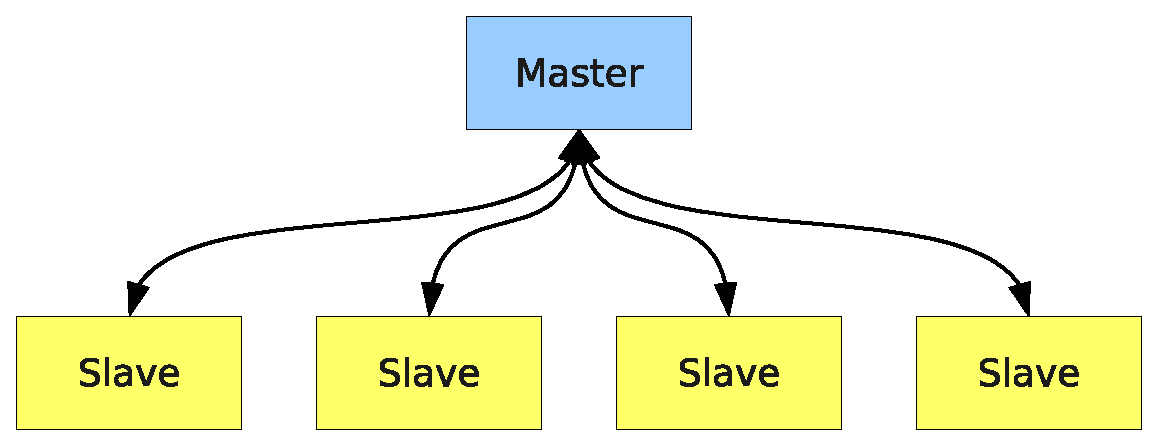
\includegraphics[width=0.9\textwidth]{figures/master-slave/master-slave.eps}
  \caption{Typical master-slave algorithm.}
  \label{fig:master-slave}
\end{figure}

Eigenvalue calculations are slightly more difficult to parallelize
than fixed source calculations since it is necessary to converge on
the fission source distribution and eigenvalue before tallying. In a
Monte Carlo eigenvalue calculation, a finite number of neutron
histories, $N$, are tracked through their lifetime iteratively. If
fission occurs, rather than tracking the resulting fission neutrons,
the site is banked for use in the subsequent cycle. At the end of each
cycle, $N$ source sites for the next cycle must be randomly sampled
from the $M$ fission sites that were banked to ensure that the neutron
population does not grow exponentially. To ensure that the results are
reproducible, one must guarantee that the process by which fission
sites are randomly sampled does not depend on the number of
processors. What is typically done is the following \cite{mcnp}:

\begin{enumerate}
\item Each compute node \emph{send}s its fission bank sites to a
  master process;
\item The master process sorts or orders \cite{brown-sort} the fission
  sites based on a unique identifier;
\item The master process samples $N$ fission sites from the ordered
  array of $M$ sites; and
\item The master process \emph{broadcast}s all the fission sites to
  the compute nodes.
\end{enumerate}

The first and last steps of this process are the major sources of
communication overhead between cycles. Since the master process must
receive $M$ fission sites from the compute nodes, the first step is
necessarily serial. This step can be completed in $O(M)$ time. The
\emph{broadcast} step can benefit from parallelization through a
tree-based algorithm. Despite this, the communication overhead is
still considerable.

To see why this is the case, it is instructive to look at a
hypothetical example. Suppose that a calculation is run with $N =
10,000,000$ neutrons across 64 compute nodes. On average, $M =
10,000,000$ fission sites will be produced. If the data for each
fission site consists of a spatial location (three 8 byte real
numbers) and a unique identifier (one 4 byte integer), the memory
required per site is 28 bytes. To \emph{broadcast} 10,000,000 source
sites to 64 nodes will thus require transferring 17.92 GB of data.
Since each compute node does not need to keep every source site in
memory, one could modify the algorithm from a \emph{broadcast} to a
\emph{scatter}. However, for practical reasons ({\em e.g.} work
self-scheduling \cite{brown-lectures}), this is normally not done in
production Monte Carlo codes.

\subsection{Novel Algorithm}
\label{sec:algorithm}

To reduce the amount of communication required in a fission bank
synchronization algorithm, it is desirable to move away from the
typical master-slave algorithm to an algorithm whereby the compute
nodes communicate with one another only as needed. This concept is
illustrated in Figure \ref{fig:slave-only}.
\begin{figure}[h!]
  \centering
  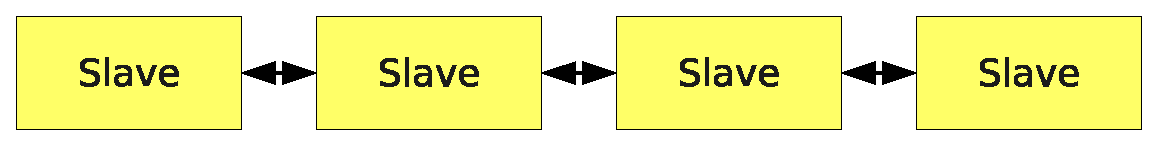
\includegraphics[width=0.9\textwidth]{figures/master-slave/slave-only.eps}
  \caption{Desired communication topology with no master process.}
  \label{fig:slave-only}
\end{figure}

Since the source sites for each cycle are sampled from the fission
sites banked from the previous cycle, it is a common occurrence for a
fission site to be banked on one compute node and sent back to the
master only to get sent back to the same compute node as a source
site. As a result, much of the communication inherent in the algorithm
described previously is entirely unnecessary. By keeping the fission
sites local, having each compute node sample fission sites, and
sending sites between nodes only as needed, one can cut down on most
of the communication. One algorithm to achieve this is as follows:

\begin{enumerate}
\item An exclusive scan is performed on the number of sites banked,
  and the total number of fission bank sites is broadcasted to all
  compute nodes. By picturing the fission bank as one large array
  distributed across multiple nodes, one can see that this step
  enables each compute node to determine the starting index of fission
  bank sites in this array. Let us call the starting and ending
  indices on the $i$-th node $a_i$ and $b_i$, respectively;
\item Each compute node samples sites at random from the fission bank
  using the same starting seed. A separate array on each compute node
  is created that consists of sites that were sampled local to that
  node, {\em i.e.} if the index of the sampled site is between $a_i$
  and $b_i$, it is set aside;
\item If any node sampled more than $N/p$ fission sites where $p$ is
  the number of compute nodes, the extra sites are put in a separate
  array and sent to all other compute nodes. This can be done
  efficiently using the \emph{allgather} collective operation;
\item The extra sites are divided among those compute nodes that
  sampled fewer than $N/p$ fission sites.
\end{enumerate}

However, even this algorithm exhibits more communication than
necessary since the \emph{allgather} will send fission bank sites to
nodes that don't necessarily need any extra sites.

One alternative is to replace the \emph{allgather} with a series of
\emph{sends}. If $a_i$ is less than $iN/p$, then send $iN/p - a_i$
sites to the left adjacent node. Similarly, if $a_i$ is greater than
$iN/p$, then receive $a_i - iN/p$ from the left adjacent node. This
idea is applied to the fission bank sites at the end of each node's
array as well. If $b_i$ is less than $(i+1)N/p$, then receive
$(i+1)N/p - b_i$ sites from the right adjacent node. If $b_i$ is
greater than $(i+1)N/p$, then send $b_i - (i+1)N/p$ sites to the right
adjacent node. Thus, each compute node sends/receives only two
messages under normal circumstances.

The following example illustrates how this algorithm works. Let us
suppose we are simulating $N = 1,000$ neutrons across four compute
nodes. For this example, it is instructive to look at the state of the
fission bank and source bank at several points in the algorithm:
\begin{enumerate}
\item The beginning of a cycle where each node has $N/p$ source sites;
\item The end of a cycle where each node has accumulated fission sites;
\item After sampling, where each node has some amount of source sites
  usually not equal to $N/p$;
\item After redistribution, each node again has $N/p$ source sites for
  the next cycle;
\end{enumerate}

At the end of each cycle, each compute node needs 250 fission bank
sites to continue on the next cycle. Let us suppose that $p_0$
produces 270 fission banks sites, $p_1$ produces 230, $p_2$ produces
290, and $p_3$ produces 250. After each node samples from its fission
bank sites, let's assume that $p_0$ has 260 source sites, $p_1$ has
215, $p_2$ has 280, and $p_3$ has 245. Note that the total number of
sampled sites is 1,000 as needed. For each node to have the same number
of source sites, $p_0$ needs to send its right-most 10 sites to $p_1$,
and $p_2$ needs to send its left-most 25 sites to $p_1$ and its
right-most 5 sites to $p_3$. A schematic of this example is shown in
Figure \ref{fig:algorithm-new}. The data local to each node is given a
different hatching, and the cross-hatched regions represent source
sites that are communicated between adjacent nodes.
\begin{figure}[h!]
  \centering
  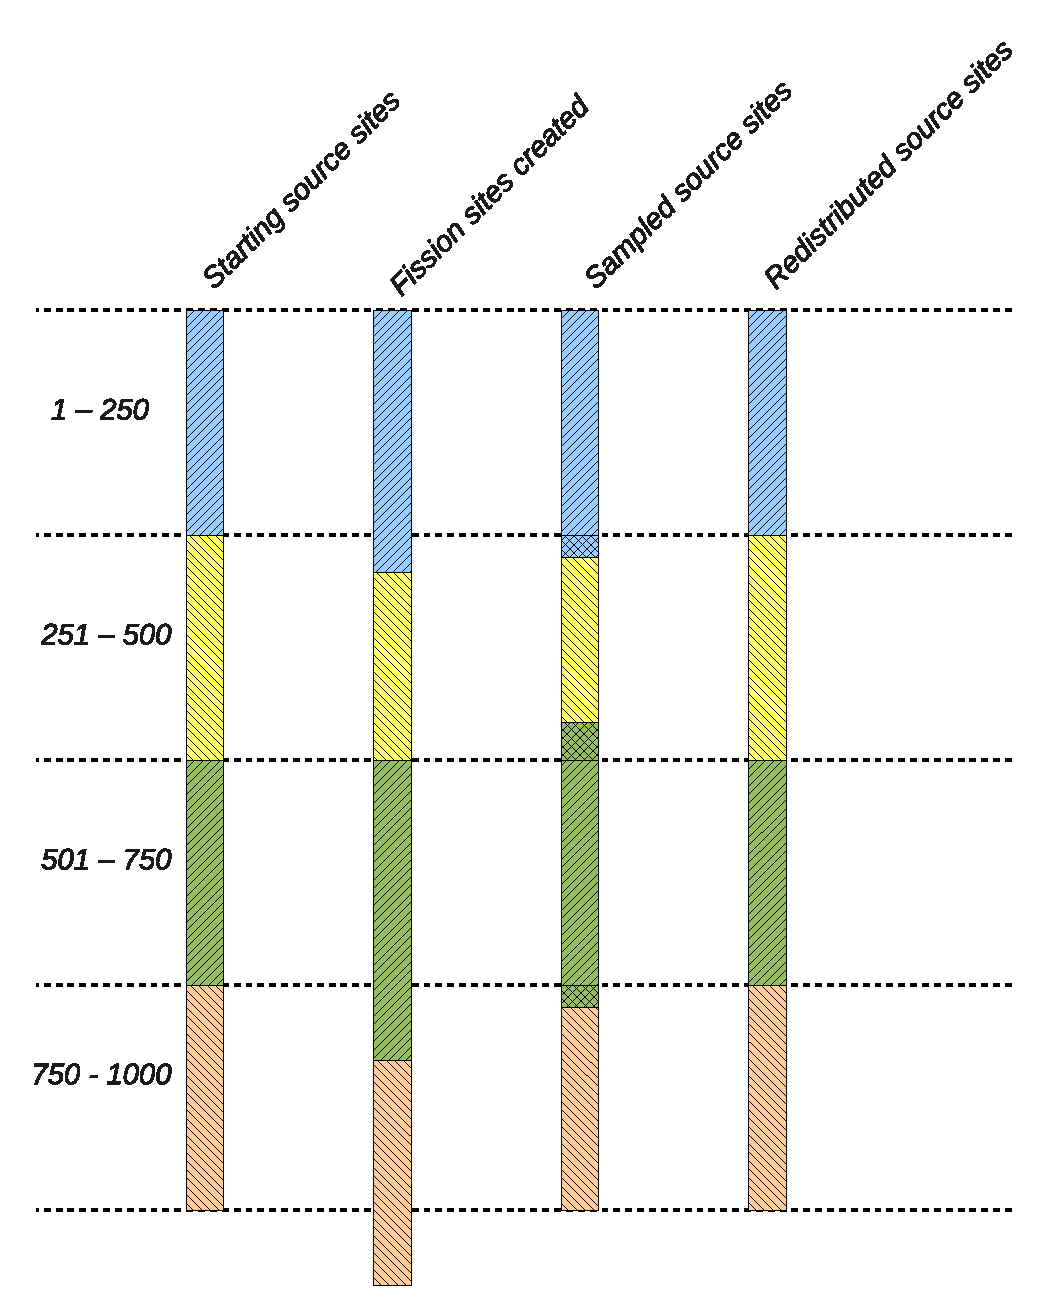
\includegraphics[width=0.9\textwidth]{figures/algorithm_schematic/algorithm-new.eps}
  \caption{Example scenario illustrating new fission bank algorithm.}
  \label{fig:algorithm-new}
\end{figure}

\section{Analysis of Communication Requirements}
\label{sec:analysis}

While the prior considerations may make it readily apparent that the
novel algorithm should outperform the traditional algorithm, it is
instructive to look at the total communication cost of the novel
algorithm relative to the traditional algorithm. This is especially so
because the novel algorithm does not have a constant communication
cost due to stochastic fluctuations. Let us begin by looking at the
cost of communication in the traditional algorithm

\subsection{Cost of Traditional Algorithm}
\label{sec:traditional-cost}

As discussed earlier, the traditional algorithm is composed of a
series of \emph{send}s and typically a \emph{broadcast}. To estimate
the communication cost of the algorithm, we can apply a simple model
that captures the essential features. In this model, we assume that
the time that it takes to send a message between two nodes is given by
$\alpha + (sN)\beta$, where $\alpha$ is the time it takes to initiate
the communication (commonly called the latency), $\beta$ is the
transfer time per unit of data, $N$ is the number of fission sites,
and $s$ is the size in bytes of each fission site.

The first step of the traditional algorithm is to send $p$ messages to
the master node, each of size $sN/p$. Thus, the total time to send
these messages is
\begin{equation}\label{eq:t-send}
  t_{\text{send}} = p\alpha + sN\beta.
\end{equation}
Generally, the best parallel performance is achieved in a weak scaling
scheme where the total number of histories is proportional to the
number of processors. However, we see that when $N$ is proportional to
$p$, the time to send these messages increases proportionally with
$p$.

Estimating the time of the \emph{broadcast} is complicated by the fact
that different MPI implementations may use different algorithms to
perform collective communications. Worse yet, a single implementation
may use a different algorithm depending on how many nodes are
communicating and the size of the message. Using multiple algorithms
allows one to minimize latency for small messages and minimize
bandwidth for long messages.

We will focus here on the implementation of \emph{broadcast} in the
MPICH2 implementation \cite{mpich}. For short messages, MPICH2 uses a
binomial tree algorithm. In this algorithm, the root process sends the
data to one node in the first step, and then in the subsequent, both
the root and the other node can send the data to other nodes. Thus, it
takes a total of $\lceil \log_2 p \rceil$ steps to complete the
communication where $\lceil x \rceil$ is the smallest integer not less
than $x$. The time to complete the communication is
\begin{equation}
  t_{\text{short}} = \lceil \log_2 p \rceil \left ( \alpha + sN\beta
  \right ).
\end{equation}
This algorithm works well for short messages since the latency term
scales logarithmically with the number of nodes. However, for long
messages, an algorithm that has lower bandwidth has been proposed by
Van de Geijn \cite{vandegeijn} and implemented in MPICH2. Rather than
using a binomial tree, the \emph{broadcast} is divided into a
\emph{scatter} and an \emph{allgather}. The time to complete the
\emph{scatter} is $ \log_2 p \: \alpha + \frac{p-1}{p} N\beta$ using a
binomial tree algorithm. The \emph{allgather} is performed using a
ring algorithm that completes in $(p-1) \alpha + \frac{p-1}{p}
N\beta$. Thus, together the time to complete the broadcast is
\begin{equation}\label{eq:t-broadcast}
  t_{\text{long}} = \left ( \log_2 p + p - 1 \right ) \alpha + 2
  \frac{p-1}{p} sN\beta.
\end{equation}
The fission bank data will generally exceed the threshold for
switching from short to long messages (typically 8 kilobytes), and
thus we will use the equation for long messages. Adding
Eq. \ref{eq:t-send} and \ref{eq:t-broadcast}, the total cost of the
series of \emph{send}s and the \emph{broadcast} is
\begin{equation}
  t_{\text{old}} = \left ( \log_2 p + 2p - 1 \right ) \alpha +
  \frac{3p-2}{p} sN\beta.
\end{equation}

\subsection{Cost of Novel Algorithm}

With the communication cost of the traditional fission bank algorithm
quantified, we now proceed to discuss the communicatin cost of the
proposed algorithm. Comparing the cost of communication of this
algorithm with the traditional algorithm is not trivial due to fact
that the cost will be a function of how many fission sites are sampled
on each node. If each node samples exactly $N/p$ sites, there will not
be communication between nodes at all. However, if any one node
samples more or less than $N/p$ sites, the deviation will result in
communication between logically adjacent nodes. To determine the
expected deviation, one can analyze the process based on the
fundamentals of the Monte Carlo process.

The steady-state neutron transport equation for a multiplying medium
can be written in the form of an eigenvalue problem \cite{lieberoth},
\begin{equation}\label{eq:NTE}
  S(\mathbf{r})= \frac{1}{k} \int F(\mathbf{r}' \rightarrow
  \mathbf{r})S(\mathbf{r}')\: d\mathbf{r},
\end{equation}
where,
\begin{align*}
  \mathbf{r} = &\: \text{spatial coordinates of phase space} \\ S
  (\mathbf{r})= &\: \text{source distribution defined as the expected
    number of neutrons} \\ &\: \text{born from fission per unit
    phase-space volume at $\mathbf{r}$} \\ F( \mathbf{r}' \rightarrow
  \mathbf{r})= &\: \text{expected number of neutrons born from fission
    per unit} \\ &\: \text{phase space volume at $\mathbf{r}$ caused
    by a neutron at $\mathbf{r}'$} \\ k = &\: \text{eigenvalue}.
\end{align*}
The fundamental eigenvalue of Eq. \eqref{eq:NTE} is known as
$k_{eff}$, but for simplicity we will simply refer to it as $k$.

In a Monte Carlo criticality simulation, the power iteration method is
applied iteratively to obtain stochastic realizations of the source
distribution and estimates of the $k$-eigenvalue. Let us define
$\hat{S}^{(m)}$ to be the realization of the source distribution at
cycle $m$ and $\hat{\epsilon}^{(m)}$ be the deviation from the
deterministic solution arising from the stochastic nature of the
tracking process. We can write the stochastic realization in terms of
the fundamental source distribution and the fluctuating component as
\cite{brissenden}
\begin{equation}\label{eq:source}
  \hat{S}^{(m)}(\mathbf{r})= N S(\mathbf{r}) + \sqrt{N}
  \hat{\epsilon}^{(m)}(\mathbf{r}),
\end{equation}
where $N$ is the number of particle histories per cycle. Without loss
of generality, we shall drop the superscript notation indicating the
cycle as it is understood that the stochastic realization is at a
particular cycle. The expected value of the stochastic source
distribution is simply
\begin{equation}
  E \left[ \hat{S}(\mathbf{r})\right] = N S (\mathbf{r})
\end{equation}
since $E \left[ \hat{\epsilon}(\mathbf{r})\right] = 0$. The noise in
the source distribution is due only to $\hat{\epsilon}(\mathbf{r})$
and thus the variance of the source distribution will be
\begin{equation}
  \text{Var} \left[ \hat{S}(\mathbf{r})\right] = N \text{Var} \left[
    \hat{\epsilon}(\mathbf{r}) \right].
\end{equation}
Lastly, the stochastic and true eigenvalues can be written as
integrals over all phase space of the stochastic and true source
distributions, respectively, as
\begin{equation}\label{eq:k_to_source}
  \hat{k} = \frac{1}{N} \int \hat{S}(\mathbf{r}) \: d\mathbf{r} \quad
  \text{and} \quad k = \int S(\mathbf{r}) \: d\mathbf{r},
\end{equation}
noting that $S(\mathbf{r})$ is $O(1)$ since the true source
distribution is not a function of $N$ (see Nease {\em et al.}
\cite{nease} for a thorough discussion). One should note that the
expected value $k$ calculated by Monte Carlo power iteration ({\em
  i.e.} the method of successive generations) will be biased from the
true fundamental eigenvalue of Eq. \ref{eq:NTE} by $O(1/N)$
\cite{brissenden}, but we will assume henceforth that the number of
particle histories per cycle is sufficiently large to neglect this
bias.

With this formalism, we now have a framework within which we can
determine the properties of the distribution of expected number of
fission sites. The explicit form of the source distribution can be
written as
\begin{equation}
  \hat{S}(\mathbf{r}) = \sum_{i=1}^{M} w_i \delta( \mathbf{r} -
  \mathbf{r}_i )
\end{equation}
where $\mathbf{r}_i$ is the spatial location of the $i$-th fission
site, $w_i$ is the statistical weight of the fission site at
$\mathbf{r}_i$ ({\em i.e.} the weight of the neutron entering into a
fission reaction), and $M$ is the total number of fission sites. It is
clear that the total weight of the fission sites is simply the
integral of the source distribution. Integrating Eq. \ref{eq:source}
over all space, we obtain
\begin{equation}
  \int \hat{S}(\mathbf{r}) \: d\mathbf{r} = N \int S(\mathbf{r}) \:
  d\mathbf{r} + \sqrt{N} \int \hat{\epsilon}(\mathbf{r}) \:
  d\mathbf{r} .
\end{equation}
Substituting the expressions for the stochastic and true eigenvalues
from Eq. \ref{eq:k_to_source}, we can relate the stochastic eigenvalue
to the integral of the noise component of the source distribution as
\begin{equation}
  N\hat{k} = Nk + \sqrt{N} \int \hat{\epsilon}(\mathbf{r}) \:
  d\mathbf{r}.
\end{equation}
Since the expected value of $\hat{\epsilon}$ is zero, the expected
value of its integral will also be zero. We thus see that the variance
of the integral of the source distribution, {\em i.e.} the variance of
the total weight of fission sites produced, is directly proportional
to the variance of the integral of the noise component. Let us call
this term $\sigma^2$ for simplicity:
\begin{equation}
  \text{Var} \left[ \int \hat{S}(\mathbf{r}) \: d\mathbf{r} \right ] =
  N \sigma^2.
\end{equation}
The actual value of $\sigma^2$ will depend on the physical nature of
the problem, whether variance reduction techniques are employed,
etc. For instance, one could surmise that for a highly scattering
problem, $\sigma^2$ would be smaller than for a highly absorbing
problem since more collisions will lead to a more precise estimate of
the source distribution. Similarly, using implicit capture should in
theory reduce the value of $\sigma^2$.

Let us now consider the case where the $N$ total histories are divided
up evenly across $p$ compute nodes. Since each node simulates $N/p$
histories, we can write the source distribution as
\begin{equation}
  \hat{S}_i(\mathbf{r})= \frac{N}{p} S(\mathbf{r}) +
  \sqrt{\frac{N}{p}} \hat{\epsilon}_i(\mathbf{r}) \quad \text{for}
  \quad i = 1, \dots, p
\end{equation}
Integrating over all space and simplifying, we can obtain an
expression for the eigenvalue on the $i$-th node:
\begin{equation}
  \hat{k}_i = k + \sqrt{\frac{p}{N}} \int \hat{\epsilon}_i(\mathbf{r})
  \: d\mathbf{r}.
\end{equation}
It is easy to show from this expression that the stochastic
realization of the global eigenvalue is merely the average of these
local eigenvalues:
\begin{equation}\label{eq:average_k_as_sum}
  \hat{k} = \frac{1}{p} \sum_{i=1}^p \hat{k}_i.
\end{equation}
As was mentioned earlier, at the end of each cycle one must sample $N$
sites from the $M$ sites that were created. Thus, the source for the
next cycle can be seen as the fission source from the current cycle
divided by the stochastic realization of the eigenvalue since it is
clear from Eq. \ref{eq:k_to_source} that $\hat{k} = M/N$. Similarly,
the number of sites sampled on each compute node that will be used for
the next cycle is
\begin{equation}\label{eq:sites_per_node}
  M_i = \frac{1}{\hat{k}} \int \hat{S}_i(\mathbf{r}) \: d\mathbf{r} =
  \frac{N}{p} \frac{\hat{k}_i}{\hat{k}}.
\end{equation}

While we know conceptually that each compute node will under normal
circumstances send two messages, many of these messages will
overlap. Rather than trying to determine the actual communication
cost, we will instead attempt to determine the maximum amount of data
being communicated from one node to another. At any given cycle, the
number of fission sites that the $j$-th compute node will send or
receive ($\Lambda_j$) is
\begin{equation}\label{eq:Lambda}
  \Lambda_j = \left | \sum_{i=1}^j M_i - \frac{jN}{p} \right |.
\end{equation}
Noting that $jN/p$ is the expected value of the summation, we can
write the expected value of $\Lambda_j$ as the mean absolute deviation
of the summation:
\begin{equation}
  E \left [ \Lambda_j \right ] = E \left [ \left | \sum_{i=1}^j M_i -
    \frac{jN}{p} \right | \right ] = \text{MD} \left [ \sum_{i=1}^j
    M_i \right ]
\end{equation}
where $\text{MD}$ indicates the mean absolute deviation of a random
variable. The mean absolute deviation is an alternative measure of
variability.

In order to ascertain any information about the mean deviation of
$M_i$, we need to know the nature of its distribution. Thus far, we
have said nothing of the distributions of the random variables in
question. The total number of fission sites resulting from the
tracking of $N$ neutrons can be shown to be normally distributed via
the Central Limit Theorem (provided that $N$ is sufficiently large)
since the fission sites resulting from each neutron are ``sampled''
from independent, identically-distributed random variables. Thus,
$\hat{k}$ and $\int \hat{S} (\mathbf{r}) \: d\mathbf{r}$ will be
normally distributed as will the individual estimates of these on each
compute node.

Next, we need to know what the distribution of $M_i$ in
Eq. \ref{eq:sites_per_node} is or, equivalently, how $\hat{k}_i /
\hat{k}$ is distributed. The distribution of a ratio of random
variables is not easy to calculate analytically, and it is not
guaranteed that the ratio distribution is normal if the numerator and
denominator are normally distributed. For example, if $X$ is a
standard normal distribution and $Y$ is also standard normal
distribution, then the ratio $X/Y$ has the standard Cauchy
distribution. The reader should be reminded that the Cauchy
distribution has no defined mean or variance. That being said, Geary
\cite{geary} has shown that, for the case of two normal distributions,
if the denominator is unlikely to assume values less than zero, then
the ratio distribution is indeed approximately normal. In our case,
$\hat{k}$ absolutely cannot assume a value less than zero, so we can
be reasonably assured that the distribution of $M_i$ will be normal.

For a normal distribution with mean $\mu$ and distribution function
$f(x)$, it can be shown that
\begin{equation}
  \int_{-\infty}^{\infty} f(x) \left | x - \mu \right | \: dx =
  \sqrt{\frac{2}{\pi} \int_{-\infty}^{\infty} f(x) \left ( x - \mu
    \right )^2 \: dx}
\end{equation}
by substituting the probability distribution function of a normal
distribution for $f(x)$, making a change of variables, and integrating
both sides. Thus the mean absolute deviation is $\sqrt{2/\pi}$ times
the standard deviation. Therefore, to evaluate the mean absolute
deviation of $M_i$, we need to first determine its
variance. Substituting Eq. \ref{eq:average_k_as_sum} in
Eq. \ref{eq:sites_per_node}, we can rewrite $M_i$ solely in terms of
$\hat{k}_1, \dots, \hat{k}_p$:
\begin{equation}
  M_i = \frac{N \hat{k}_i}{\sum\limits_{j=1}^p \hat{k}_j}.
\end{equation}
Since we know the variance of $\hat{k}_i$, we can use the error
propagation law to determine the variance of $M_i$:
\begin{equation}
  \text{Var} \left [ M_i \right ] = \sum_{j=1}^p \left (
  \frac{\partial M_i}{\partial \hat{k}_j} \right )^2 \text{Var} \left
       [ \hat{k}_j \right ] + \sum\limits_{j \neq m}
       \sum\limits_{m=1}^p \left ( \frac{\partial M_i}{\partial
         \hat{k}_j} \right ) \left ( \frac{\partial M_i}{\partial
         \hat{k}_m} \right ) \text{Cov} \left [ \hat{k}_j, \hat{k}_m
         \right ]
\end{equation}
where the partial derivatives are evaluated at $\hat{k}_j = k$. Since
$\hat{k}_j$ and $\hat{k}_m$ are independent if $j \neq m$, their
covariance is zero and thus the second term cancels out. Evaluating
the partial derivatives, we obtain
\begin{equation}
  \text{Var} \left [ M_i \right ] = \left ( \frac{N(p-1)}{kp^2} \right
  )^2 \frac{p\sigma^2}{N} + \sum_{j \neq i} \left ( \frac{-N}{kp^2}
  \right )^2 \frac{p\sigma^2}{N} = \frac{N(p-1)}{k^2p^2} \sigma^2.
\end{equation}
Through a similar analysis, one can show that the variance of
$\sum_{i=1}^j M_i$ is
\begin{equation}
  \text{Var} \left [ \sum_{i=1}^j M_i \right ] =
  \frac{Nj(p-j)}{k^2p^2} \sigma^2
\end{equation}
Thus, the expected amount of communication on node $j$, {\em i.e.} the
mean absolute deviation of $\sum_{i=1}^j M_i$ is proportional to
\begin{equation}\label{eq:comm-cost}
  E \left [ \Lambda_j \right ] = \sqrt{\frac{2Nj(p-j)\sigma^2}{\pi
      k^2p^2}}.
\end{equation}
This formula has all the properties that one would expect based on
intuition:
\begin{itemize}
\item As the number of histories increases, the communication cost on
  each node increases as well;
\item If $p=1$, {\em i.e.} if the problem is run on only one compute
  node, the variance will be zero. This reflects the fact that exactly
  $N$ sites will be sampled if there is only one node.
\item For $j=p$, the variance will be zero. Again, this says that when
  you sum the number of sites from each node, you will get exactly $N$
  sites.
\end{itemize}
We can determine the node that has the highest communication cost by
differentiating Eq. \ref{eq:comm-cost} with respect to $j$, setting it
equal to zero, and solving for $j$. Doing so yields $j_{\text{max}} =
p/2$. Interestingly, substituting $j = p/2$ in Eq. \ref{eq:comm-cost}
shows us that the maximum communication cost is actually independent
of the number of nodes:
\begin{equation}
  E \left [ \Lambda_{j_{\text{max}}} \right ] = \sqrt{
    \frac{N\sigma^2}{2\pi k^2}}.
\end{equation}

\subsection{Validation}

To ensure that any assumptions made in the foregoing analysis are
sound, several test cases were run to compare experimental results
with the theoretical analysis. The algorithm described in section
\ref{sec:algorithm} was implemented in a simple Monte Carlo code
\cite{romano-LANL}. The number of compute nodes and histories for each
case are shown in Table \ref{tab:cases}.
\begin{table}[h!]
  \centering
  \caption{Four test cases for fission bank algorithm.}
  \label{tab:cases}
  \begin{tabular}{|c|c|c|}
    \hline
    Case & Compute Nodes ($p$) & Histories ($N$) \\
    \hline
    1 & 8 & 80,000 \\
    2 & 8 & 160,000 \\
    3 & 16 & 80,000 \\
    4 & 16 & 160,000 \\
    \hline
  \end{tabular}
\end{table}
Each case was run for 10,000 cycles and at the end of each run, the
standard deviation of the number of fission bank sites sent to
neighboring nodes was determined for each node as a proxy for the
communication cost. For Case 1, the data was fit to the following
function (with the same dependence on $j$ and $p$ as in
Eq. \ref{eq:comm-cost}) using a least squares regression:
\begin{equation}\label{eq:regression}
  f(j,p,\beta) = \frac{\beta}{p} \sqrt{j(p-j)}
\end{equation}
The fitting coefficient $\beta$ was then used to predict the expected
amount of communication for the other three cases. Figure
\ref{fig:mean-deviance8} shows the expected number of fission bank
sites sent or received from neighboring compute nodes, $E \left [
  \Lambda_j \right ]$, for Cases 1 and 2 along with the least squares
regression fit based on Eq. \ref{eq:regression} for Case 1 and the
prediction for Case 2. Figure \ref{fig:mean-deviance16} shows the
expected number of fission bank sites sent or received from
neighboring compute nodes for Cases 3 and 4 along with the predicted
fits.
\begin{figure}[h!]
  \centering
  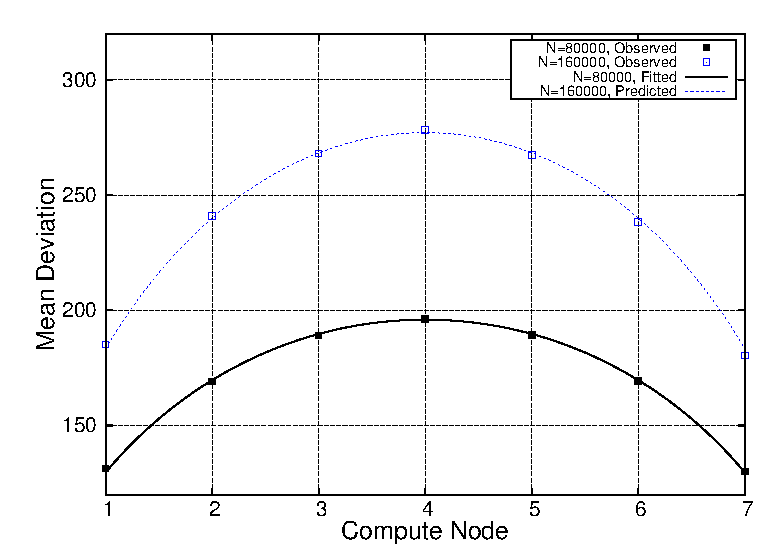
\includegraphics[width=0.75\textwidth]{figures/mean_deviance/plot8.eps}
  \caption{Expected number of fission bank sites sent to neighboring
    nodes using 8 compute nodes}
  \label{fig:mean-deviance8}
\end{figure}
\begin{figure}[h!]
  \centering
  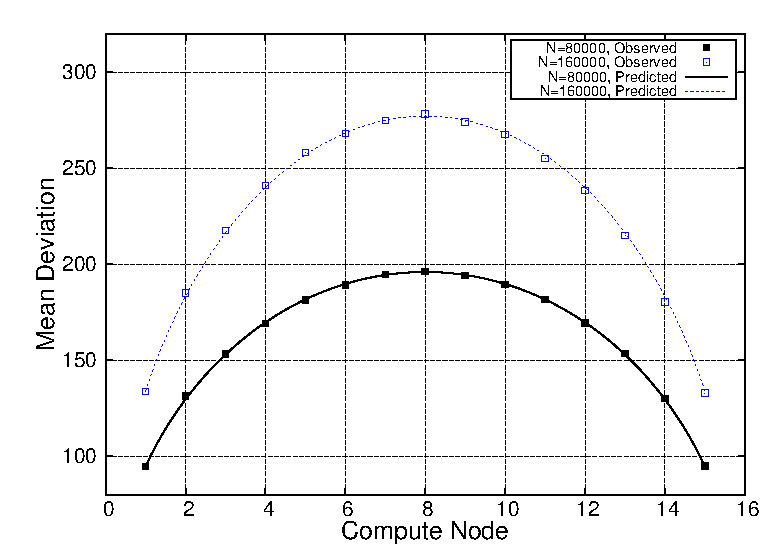
\includegraphics[width=0.75\textwidth]{figures/mean_deviance/plot16.eps}
  \caption{Expected number of fission bank sites sent to neighboring
    nodes using 16 compute nodes}
  \label{fig:mean-deviance16}
\end{figure}

A few observations can be made from these figures. Firstly, the data
from the four test cases demonstrates that the foregoing theoretical
analysis is indeed correct. Furthermore, one can observe from these
two figures that the maximum communication does occur for node
$j_{\text{max}} = p/2$ and that this maximum is indeed independent of
$p$ as predicted.

It is also instructive to check our assumption that $\sum_{i=1}^j M_i$
is normally distributed. One way of doing this is through a
quantile-quantile (Q-Q) plot, comparing the observed quantiles of the
data with the theoretical quantiles of the normal distribution. If the
data are normally distributed, the points on the Q-Q plot should lie
along a line. Figure \ref{fig:QQ-plot} shows a Q-Q plot for the number
of fission bank sites sent or received on the first node for the Case
1.
\begin{figure}[h!]
  \centering
  \includegraphics[width=0.75\textwidth,angle=-90]{figures/QQ_plot/QQplot.eps}
  \caption{Q-Q plot of $M_1$ for Case 1}
  \label{fig:QQ-plot}
\end{figure}
The data clearly lie along a straight line and thus the data are
normally distributed. This conclusion was also confirmed using the
Shapiro-Wilk test for normality \cite{shapiro-wilk}.

\subsection{Comparison of Communication Costs}

In section \ref{sec:traditional-cost}, the communication time of the
traditional fission bank algorithm was estimated using a simple model
for the transfer time based on latency and bandwidth. The same can be
done for the novel algorithm. As described earlier, each node should
send or receive only two messages, one to each of its
neighbors. Moreover, we concluded that the maximum amount of data will
be transferred for node $j_{\text{max}} = p/2$. Thus, we can estimate
the communication time for the novel algorithm as
\begin{equation}
  t_{\text{new}} = 2\alpha + s\sqrt{\frac{2N\sigma^2}{\pi k^2}} \beta
\end{equation}
To compare the communication time of the two algorithms, let us assume
that the size of the data is large enough that the latency is
negligible. The ratio of communication times is
\begin{equation}
  \frac{t_{\text{old}}}{t_{\text{new}}} = \frac{\left ( \log_2 p + 2p
    - 1 \right ) \alpha + \frac{3p-2}{p} sN\beta}{2\alpha +
    s\sqrt{\frac{2N\sigma^2}{\pi k^2}} \beta} \approx \frac{ \left (
    3p - 2 \right ) k \sqrt{N\pi/2}}{ p\sigma }.
\end{equation}
In the limit of large $p$, this ratio becomes
\begin{equation}
  \lim_{p\rightarrow\infty} \frac{t_{\text{old}}}{t_{\text{new}}} =
  \sqrt{\frac{N\pi}{2}} \cdot \frac{3k}{\sigma}.
\end{equation}
To fully appreciate what this means, we can infer values of $\sigma$
and $k$ from the aforementioned test cases to determine what the ratio
actually is. Recall that $\sigma$ tells us how much stochastic noise
there is in the integrated fission source. The sample standard
deviation for our validation cases was $\sigma = 1.73$. Using this
value and $k = 1$, we estimate that the novel algorithm would be about
2,000 times faster than the traditional algorithm for $N =
1,000,000$. Also note that as $N$ increases, the novel algorithm will
outperform the traditional algorithm by an even wider margin.

To determine the actual performance of the novel algorithm relative to
the traditional algorithm, both algorithms were implemented in the
aforementioned simple Monte Carlo code. A separate simulation using
each of the algorithms was run from a single compute node up to 88
compute nodes in parallel. In each case, the number of histories was
40,000 times the number of compute nodes so that each compute node
simulates the same number of histories. Each simulation was run for 20
cycles. Figure \ref{fig:algorithm-time} shows the total time spent on
fission bank synchronization for the traditional and novel algorithms.
\begin{figure}[h!]
  \centering
  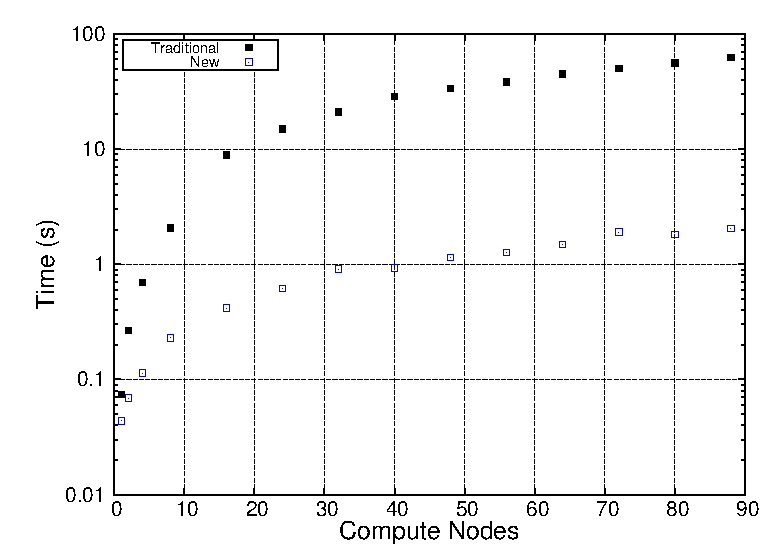
\includegraphics[width=0.75\textwidth]{figures/algorithm_results/time.eps}
  \caption{Execution time for fission bank algorithms}
  \label{fig:algorithm-time}
\end{figure}
We see that the performance of the novel algorithm doesn't quite meet
the predicted performance based on the above analysis, but this is not
surprising given the number of simplifying assumptions made in the
course of the analysis. Most importantly, we have ignored the time
spent sampling fission sites and copying data in memory which may
become non-negligible for large $N$. Notwithstanding, the new
algorithm performs nearly two orders of magnitude faster than the
traditional algorithm for large $p$ and large $N$.

\section{Other Considerations}
\label{sec:other}

A discussion of any parallel algorithm for Monte Carlo codes would not
be complete without considering how to achieve high parallel
efficiency on heterogeneous architectures and how to maintain
reproducibility of results. In this section, we will discuss how load
balancing requirements may affect the proposed algorithm and
reproducibility as well as briefly mentioning the impact of fault
tolerance.

\subsection{Load Balancing}
\label{load-balancing}

One important requirement for a parallel Monte Carlo calculation is
proper load-balancing, {\em i.e.} it is undesirable to have a compute
node sitting idle with no work to do while other compute nodes are
still busy working. This is especially the case when the hardware
architecture is heterogeneous (having different types of processors in
a single cluster). In the traditional parallel algorithm, work
self-scheduling is achieved by having each slave node request small
batches of work from the master, and as each batch is completed, the
slave may request more work. By breaking up the problem into smaller
batches, this ensures that in a single source iteration, a processor
that is twice as fast as another processor will also be assigned twice
as many histories to compute, and thus all processors should finish
their work at approximately the same time (assuming that the time to
complete a single history is constant irrespective of its properties).

The novel algorithm we have presented here precludes the use of the
aforementioned self-scheduling algorithm since an important aspect of
the algorithm is to assign histories sequentially to the nodes to
preserve their order. It should be noted that if one did not care to
preserve reproducibility in a calculation, the self-scheduling scheme
could easily be applied for load-balancing with the new fission bank
algorithm.

When used on a homogeneous cluster, we don't foresee a great loss in
efficiency due to the lack of load balancing in the novel
algorithm. Studies using MCNP on a homogeneous Linux cluster have
shown a 5-10\% loss in parallel efficiency when not using any sort of
load balancing \cite{brown-lectures}.

It is also possible to employ a basic means of load balancing for
heterogeneous architectures in the fission bank algorithm presented
here by ``tuning'' the algorithm to the specific characteristics of
the cluster. If one were to measure the performance of each type of
processor on the cluster in terms of particles processed per second,
the number of histories on each processor could be adjusted
accordingly instead of merely distributing particles uniformly ($N/p$
on each processor).

\subsection{Ordering of the Fission Bank}

The order of the fission sites produced at the end of a source
iteration will depend on the order in which the particle histories
were processed. Thus, if a calculation is run in parallel using the
master-slave load balancing scheme described above, the order of the
fission sites is not guaranteed to be reproducible since the order in
which the particle histories are simulated will depend on the actions
of independent processors. It is thus necessary to sort or re-order
the fission sites since the sampling of source sites depends on this
ordering in order to obtain a reproducible result.

A traditional sorting of the fission bank would be done using a
standard quicksort that can be completed in $O(N \log N)$ steps. Brown
and Sutton developed a method of re-ordering the fission sites that
can be done in $O(N)$ steps \cite{brown-sort}. Anecdotally, we have
observed that in systems using a high-speed network interconnect such
as InfiniBand, the sorting of the fission bank is the major
contributor to decreased parallel efficiency in fission bank
synchronization.

Using the fission bank algorithm we have developed herein, the order
in which particle histories are processed is always the same since we
simply allocate the first set of $N/p$ particles to the first
processor, the second set of $N/p$ particles to the second processor,
etc. Thus, it is not necessary to sort or re-order the fission bank in
order to preserve reproducibility of results.

\subsection{Fault Tolerance}

On a parallel architecture with a large number of processors, network
interconnects, hard disks, and memory, it is desirable to have some
means of fault tolerance to ensure that not all results are lost in
the event of a hardware failure. In current Monte Carlo codes, this
can be achieved by having the slave nodes periodically rendezvous and
having a single processor dump data to a file that can be used to
restart the run. While providing insurance against lost simulation
time, performing fault tolerance this way unfortunately degrades
parallel performance since it entails collective communication between
all processors. Notwithstanding, the algorithm we have presented here
does not inhibit the use of fault tolerance in this manner.

\section{Conclusions}
\label{sec:conclusions}

We have presented a new method for parallelizing the source iterations
in a Monte Carlo criticality calculation. This algorithm takes
advantage of the fact that many of the fission sites produced on one
processor can be used as source sites on that same processor and
avoids unnecessary communication between processors.

Analysis of the algorithm shows that it should outperform existing
algorithms for fission bank synchronization and that furthermore, the
performance gap increases for an increasing number of histories or
processors. Test results on a simple 3D structured mesh Monte Carlo
code confirm this finding. The analysis also shows that the maximum
amount of communication in the algorithm is independent of the number
of processors and instead will depend on the number of histories per
cycle and the physical characteristics of the problem at hand. Again,
testing using our simple Monte Carlo code confirm this prediction.

The reader should keep in mind that while the algorithm presented here
will significantly improve the time necessary to sample and distribute
fission sites between cycles, it has no effect on the actual transport
simulation of particles moving through a geometry. Thus, it will not
improve smaller simulations that would typically run on a
workstation. However, for large simulations that necessitate the use
of a large cluster or supercomputer to complete in a reasonable amount
of time, this novel algorithm will improve the parallel efficiency and
is an important step in achieving scalability up to thousands of
processors.

Potential shortcomings of the present algorithm include the inability
to provide load balancing using existing algorithms for heterogeneous
computer architectures. A basic method to provide load balancing in
such situations based on ``tuning'' the algorithm was suggested,
although it has not be tested as of yet.
